\section{\textcolor{unibablueI}{Sponsors}}
\begin{center}
\begin{tikzpicture}[yscale=-0.1, xscale=0.1, node distance=1mm,outer sep = 0pt]
\tikzset{grid/.style={gray,very thin,opacity=1}}
\tikzstyle{default}=[anchor=center]
    
%\draw[grid] (0,0) grid (10*\textwidth,10*\textheight);
\node[default] at (30,10) {
        
\includegraphics[width=.6\textwidth]{images/sterhard.pdf}
    };
\end{tikzpicture}
\end{center}

\begin{center}
%  
% 
 \begin{tikzpicture}[yscale=-0.1, xscale=0.1, node distance=3mm,outer sep = 0pt, inner sep=0pt]
\tikzset{grid/.style={gray,very thin,opacity=1}}
\tikzstyle{default}=[anchor=north west]
\tikzstyle{bg}=[fill=unibayellowV, opacity=.75, anchor=north west]    

\draw[bg, rounded corners] (0,0) rectangle (10*\textwidth,21);
%\draw[grid] (0,0) grid (10*\textwidth,3*\textheight);
\node[default] (gi) at (2,2) {
        
\includegraphics[width=.2\textwidth]{images/gi.png}
    };
\node[default] (itg) [right=of gi] {
        
\includegraphics[width=.25\textwidth]{images/itg.png}
    };
\node[default] (dft) [right=of itg] {
        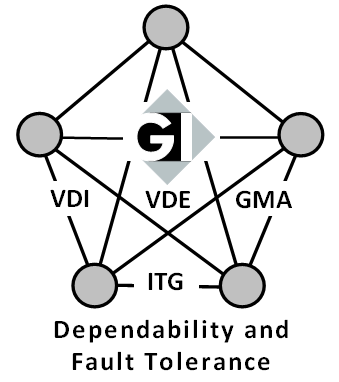
\includegraphics[width=.2\textwidth]{images/dft.png}
    };
\node[default] (mmb) [right=of dft] {
        
\includegraphics[width=.2\textwidth]{images/mmb.png}
    };
\end{tikzpicture} 
 \end{center}